% !TeX root = ..\main.tex
\appendix
\uselandscape
	\chapter{Ergebnisse des Benchmarks} \label{apx:benchmark-results}
	
	\section{HTTP-Server} \label{sec:benchmark-results-http-server}
	\begin{longtable}{
			c
			S[table-format=6.2]
			S[table-format=2.2]
			S[table-format=3.0]
			S[table-format=3]
			S[table-format=2.0]
			S[table-format=4.0]
		}
		\caption[HTTP-Server - Ergebnisse von Bun auf macOS]{HTTP-Server - Ergebnisse von Bun auf macOS\protect\linebreak\textit{Quelle: Eigene Darstellung}}
		\label{tab:http-macos-bun}
		\\
		\toprule
		Nr. & {Req/s} & {Durchschn. Latenz (ms)} & {Max. Latenz (ms)} & {Erfolgr. Req (\%)} & {Max. CPU-Ausl. (\%)} & {Max. RAM (kB)} \\
		\midrule
		\endfirsthead
		\toprule
		Nr. & {Req/s} & {Durchschn. Latenz (ms)} & {Max. Latenz (ms)} & {Erfolgr. Req (\%)} & {Max. CPU-Ausl. (\%)} & {Max. RAM (kB)} \\
		\midrule
		\endhead
		1 & 75482.69 & 6.62 & 191 & 100 & 83 & 28928 \\
		2 & 75978.26 & 6.58 & 162 & 100 & 83 & 28960 \\
		3 & 76467.36 & 6.54 & 168 & 100 & 81 & 28832 \\
		4 & 72942.36 & 6.85 & 123 & 100 & 83 & 28992 \\
		5 & 77558.43 & 6.45 & 194 & 100 & 83 & 28800 \\
		Durchschnitt & 75685.82 & 6.61 & 167.7 & 100 & 82.6 & 28902.4 \\
		\bottomrule
	\end{longtable}
	
	\begin{longtable}{
			c
			S[table-format=6.2]
			S[table-format=2.2]
			S[table-format=3.0]
			S[table-format=3]
			S[table-format=2.0]
			S[table-format=4.0]
		}
		\caption[HTTP-Server - Ergebnisse von Node.js LTS auf macOS]{HTTP-Server - Ergebnisse von Node.js LTS auf macOS\protect\linebreak\textit{Quelle: Eigene Darstellung}}
		\label{tab:http-macos-nodejs-lts}
		\\
		\toprule
		Nr. & {Req/s} & {Durchschn. Latenz (ms)} & {Max. Latenz (ms)} & {Erfolgr. Req (\%)} & {Max. CPU-Ausl. (\%)} & {Max. RAM (kB)} \\
		\midrule
		\endfirsthead
		\toprule
		Nr. & {Req/s} & {Durchschn. Latenz (ms)} & {Max. Latenz (ms)} & {Erfolgr. Req (\%)} & {Max. CPU-Ausl. (\%)} & {Max. RAM (kB)} \\
		\midrule
		\endhead
		1 & 46037.35 & 10.36 & 180 & 100 & 84 & 93536 \\
		2 & 46323.8 & 10.86 & 202 & 100 & 84 & 94432 \\
		3 & 45762.3 & 10.92 & 199 & 100 & 85 & 93456 \\
		4 & 45035.39 & 11.1 & 195 & 100 & 86 & 93584 \\
		5 & 45776.81 & 10.92 & 144 & 100 & 85 & 94016 \\
		Durchschnitt & 45787.13 & 10.83 & 184.6 & 100 & 84.8 & 93804.8 \\
		\bottomrule
	\end{longtable}
	
	\begin{longtable}{
			c
			S[table-format=6.2]
			S[table-format=2.2]
			S[table-format=3.0]
			S[table-format=3]
			S[table-format=2.0]
			S[table-format=4.0]
		}
		\caption[HTTP-Server - Ergebnisse von Node.js Latest auf macOS]{HTTP-Server - Ergebnisse von Node.js Latest auf macOS\protect\linebreak\textit{Quelle: Eigene Darstellung}}
		\label{tab:http-macos-nodejs-latest}
		\\
		\toprule
		Nr. & {Req/s} & {Durchschn. Latenz (ms)} & {Max. Latenz (ms)} & {Erfolgr. Req (\%)} & {Max. CPU-Ausl. (\%)} & {Max. RAM (kB)} \\
		\midrule
		\endfirsthead
		\toprule
		Nr. & {Req/s} & {Durchschn. Latenz (ms)} & {Max. Latenz (ms)} & {Erfolgr. Req (\%)} & {Max. CPU-Ausl. (\%)} & {Max. RAM (kB)} \\
		\midrule
		\endhead
		1 & 45680.37 & 10.94 & 1840 & 100 & 86 & 85584 \\
		2 & 45880.89 & 10.89 & 1860 & 100 & 86 & 85520 \\
		3 & 45939.12 & 10.88 & 1570 & 100 & 85 & 84386 \\
		4 & 45932.14 & 10.88 & 1650 & 100 & 86 & 83616 \\
		5 & 45974.99 & 10.87 & 1120 & 100 & 85 & 85680 \\
		Durchschnitt & 45881.502 & 10.892 & 1608 & 100 & 85.6 & 84957.2 \\
		\bottomrule
	\end{longtable}
	
	\begin{longtable}{
			c
			S[table-format=6.2]
			S[table-format=2.2]
			S[table-format=3.0]
			S[table-format=3]
			S[table-format=2.0]
			S[table-format=5.1]
		}
		\caption[HTTP-Server - Ergebnisse von Bun auf Ubuntu 23.10]{HTTP-Server - Ergebnisse von Bun auf Ubuntu 23.10\protect\linebreak\textit{Quelle: Eigene Darstellung}}
		\label{tab:http-ubuntu-bun}
		\\
		\toprule
		Nr. & {Request/s} & {Durchschn. Latenz (ms)} & {Max. Latenz (ms)} & {Erfolgr. Req (\%)} & {Max. CPU-Ausl. (\%)} & {Max. RAM (kB)} \\
		\midrule
		\endfirsthead
		\toprule
		Nr. & {Request/s} & {Durchschn. Latenz (ms)} & {Max. Latenz (ms)} & {Erfolgr. Req (\%)} & {Max. CPU-Ausl. (\%)} & {Max. RAM (kB)} \\
		\midrule
		\endhead
		1 & 103290.25 & 4.84 & 92.06 & 100 & 89 & 47188 \\
		2 & 102852.75 & 4.86 & 120.86 & 100 & 97 & 47608 \\
		3 & 102414.8 & 4.88 & 98.6 & 100 & 96 & 49392 \\
		4 & 103809.8 & 4.81 & 104.46 & 100 & 98 & 47260 \\
		5 & 103707.81 & 4.82 & 99.36 & 100 & 97 & 48484 \\
		Durchschnitt & 103215.082 & 4.842 & 103.068 & 100 & 95.4 & 47986.4 \\
		\bottomrule
	\end{longtable}
	
	\begin{longtable}{
			c
			S[table-format=6.2]
			S[table-format=2.2]
			S[table-format=3.0]
			S[table-format=3]
			S[table-format=2.0]
			S[table-format=5.1]
		}
		\caption[HTTP-Server - Ergebnisse von Node.js LTS auf Ubuntu 23.10]{HTTP-Server - Ergebnisse von Node.js LTS auf Ubuntu 23.10\protect\linebreak\textit{Quelle: Eigene Darstellung}}
		\label{tab:http-ubuntu-nodejs-lts}
		\\
		\toprule
		Nr. & {Request/s} & {Durchschn. Latenz (ms)} & {Max. Latenz (ms)} & {Erfolgr. Req (\%)} & {Max. CPU-Ausl. (\%)} & {Max. RAM (kB)} \\
		\midrule
		\endfirsthead
		\toprule
		Nr. & {Request/s} & {Durchschn. Latenz (ms)} & {Max. Latenz (ms)} & {Erfolgr. Req (\%)} & {Max. CPU-Ausl. (\%)} & {Max. RAM (kB)} \\
		\midrule
		\endhead
		1 & 30421.51 & 16.44 & 230.8 & 100 & 96 & 93856 \\
		2 & 30448.93 & 16.42 & 208.43 & 100 & 96 & 93212 \\
		3 & 29999.89 & 16.67 & 215.64 & 100 & 95 & 93144 \\
		4 & 30122.16 & 16.59 & 176.54 & 100 & 94 & 92928 \\
		5 & 30488.92 & 16.39 & 199.07 & 100 & 96 & 93116 \\
		Durchschnitt & 30296.282 & 16.502 & 206.096 & 100 & 95.4 & 93251.2 \\
		\bottomrule
	\end{longtable}
	
	\begin{longtable}{
			c
			S[table-format=6.2]
			S[table-format=2.2]
			S[table-format=3.0]
			S[table-format=3]
			S[table-format=2.0]
			S[table-format=5.1]
		}
		\caption[HTTP-Server - Ergebnisse von Node.js Latest auf Ubuntu 23.10]{HTTP-Server - Ergebnisse von Node.js Latest auf Ubuntu 23.10\protect\linebreak\textit{Quelle: Eigene Darstellung}}
		\label{tab:http-ubuntu-nodejs-current}
		\\
		\toprule
		Nr. & {Request/s} & {Durchschn. Latenz (ms)} & {Max. Latenz (ms)} & {Erfolgr. Req (\%)} & {Max. CPU-Ausl. (\%)} & {Max. RAM (kB)} \\
		\midrule
		\endfirsthead
		\toprule
		Nr. & {Request/s} & {Durchschn. Latenz (ms)} & {Max. Latenz (ms)} & {Erfolgr. Req (\%)} & {Max. CPU-Ausl. (\%)} & {Max. RAM (kB)} \\
		\midrule
		\endhead
		1 & 32358.13 & 15.45 & 7960 & 100 & 100 & 86652 \\
		2 & 31700.99 & 15.78 & 8340 & 100 & 90 & 86396 \\
		3 & 32244.05 & 15.51 & 9280 & 100 & 95 & 86280 \\
		4 & 32856.68 & 15.21 & 8210 & 100 & 99 & 86284 \\
		5 & 32269.21 & 15.5 & 8440 & 100 & 98 & 86636 \\
		Durchschnitt & 32285.812 & 15.49 & 8446 & 100 & 96.4 & 86449.6 \\
		\bottomrule
	\end{longtable}
	\newpage
	
	\section{Datei-Server} \label{sec:benchmark-results-file-server}
	
	\begin{longtable}{
			c
			S[table-format=6.2]
			S[table-format=2.2]
			S[table-format=3.2]
			S[table-format=3]
			S[table-format=2.0]
			S[table-format=5.0]
		}
		\caption[Datei-Server - Ergebnisse von Bun auf Ubuntu 23.10]{Datei-Server - Ergebnisse von Bun auf Ubuntu 23.10\protect\linebreak\textit{Quelle: Eigene Darstellung}}
		\label{tab:file-ubuntu-bun}
		\\
		\toprule
		\multicolumn{7}{c}{50 Benutzer} \\
		Nr. & {Request/s} & {Durchschn. Latenz (ms)} & {Max. Latenz (ms)} & {Erfolgr. Req (\%)} & {Max. CPU-Ausl. (\%)} & {Max. RAM (kB)} \\
		\midrule
		\endfirsthead
		\toprule
		\multicolumn{7}{c}{50 Benutzer} \\
		Nr. & {Request/s} & {Durchschn. Latenz (ms)} & {Max. Latenz (ms)} & {Erfolgr. Req (\%)} & {Max. CPU-Ausl. (\%)} & {Max. RAM (kB)} \\
		\midrule
		\endhead
		1 & 24555.25 & 2.03 & 25.73 & 100 & 98 & 83484 \\
		2 & 24688.31 & 2.02 & 40.45 & 100 & 100 & 82824 \\
		3 & 25083.61 & 1.99 & 30.04 & 100 & 98 & 83876 \\
		4 & 24978.84 & 2 & 25.65 & 100 & 101 & 83756 \\
		5 & 24503.56 & 2.04 & 29.26 & 100 & 98 & 82056 \\
		Durchschnitt & 24761.91 & 2.02 & 30.23 & 100.00 & 99.00 & 83199.20 \\
		\midrule
		\multicolumn{7}{c}{250 Benutzer} \\
		Nr. & {Request/s} & {Durchschn. Latenz (ms)} & {Max. Latenz (ms)} & {Erfolgr. Req (\%)} & {Max. CPU-Ausl. (\%)} & {Max. RAM (kB)} \\
		\midrule
		1 & 24585.85 & 10.17 & 100.97 & 100 & 98 & 82372 \\
		2 & 24988.13 & 10 & 96.19 & 100 & 97 & 83272 \\
		3 & 24290.11 & 10.29 & 73.98 & 100 & 97 & 83132 \\
		4 & 24399.87 & 10.24 & 105.26 & 100 & 98 & 82808 \\
		5 & 24926.9 & 10.03 & 80.57 & 100 & 97 & 84088 \\
		Durchschnitt & 24638.17 & 10.15 & 91.39 & 100.00 & 97.40 & 83134.40 \\
		\midrule
		\multicolumn{7}{c}{500 Benutzer} \\
		Nr. & {Request/s} & {Durchschn. Latenz (ms)} & {Max. Latenz (ms)} & {Erfolgr. Req (\%)} & {Max. CPU-Ausl. (\%)} & {Max. RAM (kB)} \\
		\midrule
		1 & 23899.18 & 20.91 & 116.19 & 100 & 96 & 82128 \\
		2 & 24201.74 & 20.65 & 108.4 & 100 & 96 & 83196 \\
		3 & 24153.93 & 20.69 & 115.38 & 100 & 100 & 82692 \\
		4 & 23658.7 & 21.12 & 119.64 & 100 & 98 & 82672 \\
		5 & 24399.08 & 20.5 & 117.62 & 100 & 99 & 82948 \\
		Durchschnitt & 24155.31 & 20.69 & 116.36 & 100.00 & 98.40 & 83124.80 \\
		\midrule
		\multicolumn{7}{c}{1000 Benutzer} \\
		Nr. & {Request/s} & {Durchschn. Latenz (ms)} & {Max. Latenz (ms)} & {Erfolgr. Req (\%)} & {Max. CPU-Ausl. (\%)} & {Max. RAM (kB)} \\
		\midrule
		1 & 23963.96 & 41.81 & 1230 & 100 & 98 & 82180 \\
		2 & 23684.71 & 42.25 & 1160 & 100 & 95 & 81876 \\
		3 & 23702.16 & 42.25 & 1170 & 100 & 93 & 83052 \\
		4 & 23546.82 & 42.53 & 1160 & 100 & 98 & 82880 \\
		5 & 24036.35 & 41.63 & 1130 & 100 & 97 & 83320 \\
		Durchschnitt & 23786.80 & 42.09 & 1170.00 & 100.00 & 96.20 & 82661.60 \\
		\bottomrule
	\end{longtable}
	
	\begin{longtable}{
			c
			S[table-format=6.2]
			S[table-format=2.2]
			S[table-format=3.2]
			S[table-format=3]
			S[table-format=2.0]
			S[table-format=5.0]
		}
		\caption[Datei-Server - Ergebnisse von Node.js LTS auf Ubuntu 23.10]{Datei-Server - Ergebnisse von Node.js LTS auf Ubuntu 23.10\protect\linebreak\textit{Quelle: Eigene Darstellung}}
		\label{tab:file-ubuntu-nodejs-lts}
		\\
		\toprule
		\multicolumn{7}{c}{50 Benutzer} \\
		Nr. & {Request/s} & {Durchschn. Latenz (ms)} & {Max. Latenz (ms)} & {Erfolgr. Req (\%)} & {Max. CPU-Ausl. (\%)} & {Max. RAM (kB)} \\
		\midrule
		\endfirsthead
		\toprule
		\multicolumn{7}{c}{50 Benutzer} \\
		Nr. & {Request/s} & {Durchschn. Latenz (ms)} & {Max. Latenz (ms)} & {Erfolgr. Req (\%)} & {Max. CPU-Ausl. (\%)} & {Max. RAM (kB)} \\
		\midrule
		\endhead
		1 & 11853.46 & 4.22 & 78.54 & 100 & 137 & 69480 \\
		2 & 11924.96 & 4.08 & 71.56 & 100 & 135 & 71184 \\
		3 & 12253.47 & 4.08 & 71.51 & 100 & 135 & 74640 \\
		4 & 11806.59 & 4.23 & 64.23 & 100 & 134 & 71224 \\
		5 & 11819.12 & 4.23 & 73.19 & 100 & 133 & 76260 \\
		Durchschnitt & 11931.52 & 4.17 & 71.81 & 100.00 & 134.80 & 72557.60 \\
		\midrule
		\multicolumn{7}{c}{250 Benutzer} \\
		Nr. & {Request/s} & {Durchschn. Latenz (ms)} & {Max. Latenz (ms)} & {Erfolgr. Req (\%)} & {Max. CPU-Ausl. (\%)} & {Max. RAM (kB)} \\
		\midrule
		1 & 9454.04 & 26.38 & 249.57 & 100 & 169 & 115504 \\
		2 & 9395.36 & 26.55 & 221.37 & 100 & 169 & 121036 \\
		3 & 9276.2 & 26.89 & 215.68 & 100 & 173 & 112908 \\
		4 & 9379.2 & 26.59 & 192.39 & 100 & 167 & 122620 \\
		5 & 9362.02 & 26.64 & 223.04 & 100 & 171 & 114472 \\
		Durchschnitt & 9373.36 & 26.61 & 220.41 & 100.00 & 169.80 & 117308.00 \\
		\midrule
		\multicolumn{7}{c}{500 Benutzer} \\
		Nr. & {Request/s} & {Durchschn. Latenz (ms)} & {Max. Latenz (ms)} & {Erfolgr. Req (\%)} & {Max. CPU-Ausl. (\%)} & {Max. RAM (kB)} \\
		\midrule
		1 & 7650.31 & 64.53 & 287.7 & 100 & 166 & 105356 \\
		2 & 8460.46 & 58.41 & 305.46 & 100 & 176 & 106928 \\
		3 & 8428.35 & 58.51 & 285.69 & 100 & 166 & 103704 \\
		4 & 8292.37 & 59.61 & 313.21 & 100 & 171 & 106108 \\
		5 & 8410.83 & 58.73 & 292.88 & 100 & 165 & 104264 \\
		Durchschnitt & 8398.00 & 58.82 & 299.31 & 100.00 & 169.50 & 105251.00 \\
		\midrule
		\multicolumn{7}{c}{1000 Benutzer} \\
		Nr. & {Request/s} & {Durchschn. Latenz (ms)} & {Max. Latenz (ms)} & {Erfolgr. Req (\%)} & {Max. CPU-Ausl. (\%)} & {Max. RAM (kB)} \\
		\midrule
		1 & 8491.34 & 118.31 & 1260 & 100 & 170 & 140472 \\
		2 & 7656.16 & 130.42 & 1260 & 100 & 178 & 143180 \\
		3 & 7714.78 & 129.42 & 1270 & 100 & 160 & 178588 \\
		4 & 8174.67 & 123.02 & 1270 & 100 & 152 & 149484 \\
		5 & 7698.82 & 129.62 & 1260 & 100 & 177 & 147612 \\
		Durchschnitt & 7947.15 & 126.16 & 1264.00 & 100.00 & 167.40 & 151867.20 \\
		\bottomrule
	\end{longtable}
	
	\begin{longtable}{
			c
			S[table-format=6.2]
			S[table-format=2.2]
			S[table-format=3.2]
			S[table-format=3]
			S[table-format=2.0]
			S[table-format=6.0]
		}
		\caption[Datei-Server - Ergebnisse von Node.js Latest auf Ubuntu 23.10]{Datei-Server - Ergebnisse von Node.js Latest auf Ubuntu 23.10\protect\linebreak\textit{Quelle: Eigene Darstellung}}
		\label{tab:file-ubuntu-nodejs-latest}
		\\
		\toprule
		\multicolumn{7}{c}{50 Benutzer} \\
		Nr. & {Request/s} & {Durchschn. Latenz (ms)} & {Max. Latenz (ms)} & {Erfolgr. Req (\%)} & {Max. CPU-Ausl. (\%)} & {Max. RAM (kB)} \\
		\midrule
		\endfirsthead
		\toprule
		\multicolumn{7}{c}{50 Benutzer} \\
		Nr. & {Request/s} & {Durchschn. Latenz (ms)} & {Max. Latenz (ms)} & {Erfolgr. Req (\%)} & {Max. CPU-Ausl. (\%)} & {Max. RAM (kB)} \\
		\midrule
		\endhead
		1 & 14237.06 & 3.51 & 116.84 & 100 & 174 & 88056 \\
		2 & 14305.85 & 3.49 & 135.14 & 100 & 194 & 84784 \\
		3 & 14685.7 & 3.4 & 146.92 & 100 & 193 & 82028 \\
		4 & 14253.49 & 3.51 & 161.68 & 100 & 193 & 85144 \\
		5 & 14690.78 & 3.4 & 127.55 & 100 & 197 & 86808 \\
		Durchschnitt & 14434.58 & 3.46 & 137.63 & 100.00 & 190.20 & 85364.00 \\
		\midrule
		\multicolumn{7}{c}{250 Benutzer} \\
		Nr. & {Request/s} & {Durchschn. Latenz (ms)} & {Max. Latenz (ms)} & {Erfolgr. Req (\%)} & {Max. CPU-Ausl. (\%)} & {Max. RAM (kB)} \\
		\midrule
		1 & 12075.16 & 20.7 & 860 & 100 & 222 & 128460 \\
		2 & 12006.8 & 20.81 & 816.63 & 100 & 218 & 124552 \\
		3 & 12038.16 & 20.76 & 880 & 100 & 220 & 121192 \\
		4 & 11927.89 & 20.95 & 845.54 & 100 & 221 & 121700 \\
		5 & 12158.18 & 20.56 & 860 & 100 & 221 & 121488 \\
		Durchschnitt & 12041.24 & 20.76 & 852.43 & 100.00 & 220.40 & 123478.40 \\
		\midrule
		\multicolumn{7}{c}{500 Benutzer} \\
		Nr. & {Request/s} & {Durchschn. Latenz (ms)} & {Max. Latenz (ms)} & {Erfolgr. Req (\%)} & {Max. CPU-Ausl. (\%)} & {Max. RAM (kB)} \\
		\midrule
		1 & 10322.75 & 47.96 & 1710 & 100 & 268 & 172996 \\
		2 & 10462.03 & 47.33 & 1740 & 100 & 265 & 118604 \\
		3 & 10337.76 & 47.97 & 1770 & 100 & 250 & 174576 \\
		4 & 10478.85 & 47.32 & 1740 & 100 & 264 & 175628 \\
		5 & 10254 & 48.39 & 1740 & 100 & 262 & 175036 \\
		Durchschnitt & 10383.16 & 47.75 & 1747.50 & 100.00 & 260.25 & 160961.00 \\
		\midrule
		\multicolumn{7}{c}{1000 Benutzer} \\
		Nr. & {Request/s} & {Durchschn. Latenz (ms)} & {Max. Latenz (ms)} & {Erfolgr. Req (\%)} & {Max. CPU-Ausl. (\%)} & {Max. RAM (kB)} \\
		\midrule
		1 & 8535.43 & 116.42 & 4240 & 100 & 278 & 213864 \\
		2 & 8553.51 & 116.28 & 3810 & 100 & 279 & 209776 \\
		3 & 8573.22 & 115.88 & 4240 & 100 & 277 & 209276 \\
		4 & 8655.02 & 114.96 & 4100 & 100 & 281 & 211692 \\
		5 & 8630.1 & 115.3 & 4070 & 100 & 283 & 213220 \\
		Durchschnitt & 8589.46 & 115.77 & 4092.00 & 100.00 & 279.60 & 211565.60 \\
		\bottomrule
	\end{longtable}
	
	\begin{longtable}{
			c
			S[table-format=6.2]
			S[table-format=2.2]
			S[table-format=3.2]
			S[table-format=3]
			S[table-format=2.0]
			S[table-format=6.0]
		}
		\caption[Datei-Server - Ergebnisse von Bun auf macOS]{Datei-Server - Ergebnisse von Bun auf macOS\protect\linebreak\textit{Quelle: Eigene Darstellung}}
		\label{tab:file-macos-bun-lts}
		\\
		\toprule
		\multicolumn{7}{c}{50 Benutzer} \\
		Nr. & {Request/s} & {Durchschn. Latenz (ms)} & {Max. Latenz (ms)} & {Erfolgr. Req (\%)} & {Max. CPU-Ausl. (\%)} & {Max. RAM (kB)} \\
		\midrule
		\endfirsthead
		\toprule
		\multicolumn{7}{c}{50 Benutzer} \\
		Nr. & {Request/s} & {Durchschn. Latenz (ms)} & {Max. Latenz (ms)} & {Erfolgr. Req (\%)} & {Max. CPU-Ausl. (\%)} & {Max. RAM (kB)} \\
		\midrule
		\endhead
		1 & 25276.77 & 1.98 & 18.82 & 100 & 92 & 67328 \\
		2 & 25302.77 & 1.97 & 14.4 & 100 & 94 & 65744 \\
		3 & 25293.36 & 1.98 & 14.06 & 100 & 95 & 65840 \\
		4 & 25292.46 & 1.98 & 13.51 & 100 & 93 & 65956 \\
		5 & 25330.78 & 1.97 & 16.1 & 100 & 94 & 654230 \\
		Durchschnitt & 25299.23 & 1.98 & 15.38 & 100.00 & 93.60 & 183819.60 \\
		\midrule
		\multicolumn{7}{c}{250 Benutzer} \\
		Nr. & {Request/s} & {Durchschn. Latenz (ms)} & {Max. Latenz (ms)} & {Erfolgr. Req (\%)} & {Max. CPU-Ausl. (\%)} & {Max. RAM (kB)} \\
		\midrule
		1 & 25464.61 & 9.82 & 55.58 & 100 & 89 & 66698 \\
		2 & 25435.68 & 9.83 & 52.12 & 100 & 92 & 66384 \\
		3 & 25476.74 & 9.81 & 50.91 & 100 & 93 & 66464 \\
		4 & 25372.19 & 9.85 & 49.03 & 100 & 92 & 66640 \\
		5 & 25451.01 & 9.82 & 49.88 & 100 & 93 & 66560 \\
		Durchschnitt & 25440.05 & 9.83 & 51.50 & 100.00 & 91.80 & 66549.20 \\
		\midrule
		\multicolumn{7}{c}{500 Benutzer} \\
		Nr. & {Request/s} & {Durchschn. Latenz (ms)} & {Max. Latenz (ms)} & {Erfolgr. Req (\%)} & {Max. CPU-Ausl. (\%)} & {Max. RAM (kB)} \\
		\midrule
		1 & 23707.59 & 21.08 & 195.63 & 100 & 90 & 64264 \\
		2 & 23920.81 & 20.9 & 239.5 & 100 & 86 & 65040 \\
		3 & 23909.89 & 20.9 & 204.46 & 100 & 90 & 65024 \\
		4 & 23825.78 & 20.98 & 206.59 & 100 & 89 & 64880 \\
		5 & 23879.56 & 20.93 & 220.08 & 100 & 90 & 64880 \\
		Durchschnitt & 23848.73 & 20.96 & 213.25 & 100.00 & 89.00 & 64817.60 \\
		\midrule
		\multicolumn{7}{c}{1000 Benutzer} \\
		Nr. & {Request/s} & {Durchschn. Latenz (ms)} & {Max. Latenz (ms)} & {Erfolgr. Req (\%)} & {Max. CPU-Ausl. (\%)} & {Max. RAM (kB)} \\
		\midrule
		1 & 24846.18 & 40.22 & 451.41 & 99.96 & 91 & 68192 \\
		2 & 24776.04 & 40.34 & 466.86 & 99.95 & 90 & 67472 \\
		3 & 24789.88 & 40.38 & 479.3 & 99.95 & 91 & 67280 \\
		4 & 24746.3 & 40.38 & 479.3 & 99.96 & 90 & 6824 \\
		5 & 24773.9 & 40.34 & 462.65 & 99.96 & 91 & 67952 \\
		Durchschnitt & 24786.46 & 40.33 & 467.90 & 99.96 & 90.60 & 55544.00 \\
		\bottomrule
	\end{longtable}
	
	\begin{longtable}{
			c
			S[table-format=5.2]
			S[table-format=2.2]
			S[table-format=2.2]
			S[table-format=3]
			S[table-format=3.0]
			S[table-format=6.0]
		}
		\caption[Datei-Server - Ergebnisse von Node.js LTS auf macOS]{Datei-Server - Ergebnisse von Node.js LTS auf macOS\protect\linebreak\textit{Quelle: Eigene Darstellung}}
		\label{tab:file-macos-nodejs-lts}
		\\
		\toprule
		\multicolumn{7}{c}{50 Benutzer} \\
		Nr. & {Request/s} & {Durchschn. Latenz (ms)} & {Max. Latenz (ms)} & {Erfolgr. Req (\%)} & {Max. CPU-Ausl. (\%)} & {Max. RAM (kB)} \\
		\midrule
		\endfirsthead
		\toprule
		\multicolumn{7}{c}{50 Benutzer} \\
		Nr. & {Request/s} & {Durchschn. Latenz (ms)} & {Max. Latenz (ms)} & {Erfolgr. Req (\%)} & {Max. CPU-Ausl. (\%)} & {Max. RAM (kB)} \\
		\midrule
		\endhead
		1 & 21515 & 2.32 & 33.96 & 100 & 146 & 120544 \\
		2 & 19785.3 & 2.53 & 36.05 & 100 & 142 & 125616 \\
		3 & 19363.94 & 2.58 & 33.9 & 100 & 143 & 124096 \\
		4 & 21722.08 & 2.3 & 29.84 & 100 & 143 & 109568 \\
		5 & 21449.79 & 2.33 & 33.51 & 100 & 145 & 119792 \\
		Durchschnitt & 20767.22 & 2.41 & 33.45 & 100.00 & 143.80 & 119923.20 \\
		\midrule
		\multicolumn{7}{c}{250 Benutzer} \\
		Nr. & {Request/s} & {Durchschn. Latenz (ms)} & {Max. Latenz (ms)} & {Erfolgr. Req (\%)} & {Max. CPU-Ausl. (\%)} & {Max. RAM (kB)} \\
		\midrule
		1 & 15917.54 & 15.55 & 70.35 & 100 & 193 & 195552 \\
		2 & 16075.37 & 15.51 & 81.9 & 100 & 186 & 168992 \\
		3 & 16074.26 & 15.55 & 65.21 & 100 & 189 & 191920 \\
		4 & 16111.43 & 15.51 & 81.9 & 100 & 188 & 189536 \\
		5 & 15924.32 & 15.7 & 70.46 & 100 & 191 & 176272 \\
		Durchschnitt & 16020.58 & 15.56 & 73.96 & 100.00 & 189.40 & 184454.40 \\
		\midrule
		\multicolumn{7}{c}{500 Benutzer} \\
		Nr. & {Request/s} & {Durchschn. Latenz (ms)} & {Max. Latenz (ms)} & {Erfolgr. Req (\%)} & {Max. CPU-Ausl. (\%)} & {Max. RAM (kB)} \\
		\midrule
		1 & 14317.65 & 34.93 & 248.08 & 100 & 189 & 229776 \\
		2 & 14508.2 & 34.46 & 231.62 & 100 & 197 & 198496 \\
		3 & 14466.72 & 34.56 & 214.82 & 100 & 185 & 208496 \\
		4 & 14610.55 & 34.21 & 198.59 & 100 & 176 & 212880 \\
		5 & 14647.9 & 34.12 & 238.61 & 100 & 190 & 209896 \\
		Durchschnitt & 14510.20 & 34.46 & 226.34 & 100.00 & 187.40 & 211908.80 \\
		\midrule
		\multicolumn{7}{c}{1000 Benutzer} \\
		Nr. & {Request/s} & {Durchschn. Latenz (ms)} & {Max. Latenz (ms)} & {Erfolgr. Req (\%)} & {Max. CPU-Ausl. (\%)} & {Max. RAM (kB)} \\
		\midrule
		1 & 14970.63 & 66.75 & 511.17 & 99.92 & 193 & 284000 \\
		2 & 14629.17 & 68.36 & 452.81 & 99.93 & 198 & 300096 \\
		3 & 14524.19 & 68.75 & 594.74 & 99.92 & 195 & 286704 \\
		4 & 14274.59 & 69.98 & 572.31 & 99.92 & 199 & 294704 \\
		5 & 13378.25 & 74.77 & 550.02 & 99.92 & 190 & 311296 \\
		Durchschnitt & 14355.37 & 69.72 & 536.21 & 99.92 & 195.00 & 295360.00 \\
		\bottomrule
	\end{longtable}
	
	\begin{longtable}{
			c
			S[table-format=5.2]
			S[table-format=2.2]
			S[table-format=2.2]
			S[table-format=3]
			S[table-format=3.0]
			S[table-format=6.0]
		}
		\caption[Datei-Server - Ergebnisse von Node.js Latest auf macOS]{Datei-Server - Ergebnisse von Node.js Latest auf macOS\protect\linebreak\textit{Quelle: Eigene Darstellung}}
		\label{tab:file-macos-nodejs-latest}
		\\
		\toprule
		\multicolumn{7}{c}{50 Benutzer} \\
		Nr. & {Request/s} & {Durchschn. Latenz (ms)} & {Max. Latenz (ms)} & {Erfolgr. Req (\%)} & {Max. CPU-Ausl. (\%)} & {Max. RAM (kB)} \\
		\midrule
		\endfirsthead
		\toprule
		\multicolumn{7}{c}{50 Benutzer} \\
		Nr. & {Request/s} & {Durchschn. Latenz (ms)} & {Max. Latenz (ms)} & {Erfolgr. Req (\%)} & {Max. CPU-Ausl. (\%)} & {Max. RAM (kB)} \\
		\midrule
		\endhead
		1 & 21553.66 & 2.32 & 81.25 & 100 & 146 & 117296 \\
		2 & 21499.51 & 2.32 & 61.8 & 100 & 148 & 109888 \\
		3 & 21808.63 & 2.29 & 61.93 & 100 & 146 & 112464 \\
		4 & 21799.37 & 2.29 & 63.66 & 100 & 144 & 119520 \\
		5 & 21519.05 & 2.32 & 60.17 & 100 & 148 & 115120 \\
		Durchschnitt & 21636.04 & 2.31 & 65.76 & 100.00 & 146.40 & 114857.60 \\
		\midrule
		\multicolumn{7}{c}{250 Benutzer} \\
		Nr. & {Request/s} & {Durchschn. Latenz (ms)} & {Max. Latenz (ms)} & {Erfolgr. Req (\%)} & {Max. CPU-Ausl. (\%)} & {Max. RAM (kB)} \\
		\midrule
		1 & 17388.28 & 14.38 & 469.75 & 99.99 & 190 & 203264 \\
		2 & 17301.54 & 14.45 & 484.46 & 99.99 & 191 & 202544 \\
		3 & 17374.5 & 14.39 & 455.17 & 100.00 & 186 & 184224 \\
		4 & 17193.03 & 14.54 & 478.6 & 99.99 & 186 & 208992 \\
		5 & 16918.4 & 5.55 & 492.5 & 100.00 & 187 & 198144 \\
		Durchschnitt & 17235.15 & 12.66 & 476.10 & 99.99 & 188.00 & 199433.60 \\
		\midrule
		\multicolumn{7}{c}{500 Benutzer} \\
		Nr. & {Request/s} & {Durchschn. Latenz (ms)} & {Max. Latenz (ms)} & {Erfolgr. Req (\%)} & {Max. CPU-Ausl. (\%)} & {Max. RAM (kB)} \\
		\midrule
		1 & 14790.27 & 33.81 & 1720 & 99.50 & 195 & 221728 \\
		2 & 14729.2 & 33.93 & 1790 & 99.40 & 194 & 219552 \\
		3 & 14749.95 & 33.91 & 1649 & 99.70 & 198 & 234800 \\
		4 & 14722.22 & 33.98 & 1920 & 99.40 & 193 & 243920 \\
		5 & 14628.28 & 34.14 & 1820 & 99.70 & 194 & 257200 \\
		Durchschnitt & 14723.98 & 33.95 & 1779.80 & 99.54 & 194.80 & 235440.00 \\
		\midrule
		\multicolumn{7}{c}{1000 Benutzer} \\
		Nr. & {Request/s} & {Durchschn. Latenz (ms)} & {Max. Latenz (ms)} & {Erfolgr. Req (\%)} & {Max. CPU-Ausl. (\%)} & {Max. RAM (kB)} \\
		\midrule
		1 & 14937.53 & 66.91 & 6000 & 99.87 & 210 & 283264 \\
		2 & 14518.01 & 68.83 & 5140 & 99.48 & 206 & 366512 \\
		3 & 14594.26 & 67.85 & 4350 & 99.46 & 203 & 317392 \\
		4 & 14719.55 & 68.2 & 4540 & 99.38 & 198 & 361280 \\
		5 & 14651.76 & 68.2 & 4540 & 99.50 & 206 & 323952 \\
		Durchschnitt & 14684.22 & 68.00 & 4914.00 & 99.54 & 204.60 & 330480.00 \\
		\bottomrule
	\end{longtable}
	
	\section{Berechnung der Fibonacci-Folge} \label{sec:benchmark-results-fibonacci}
	\begin{longtable}{c S[table-format=2.2] c S[table-format=5.0]}
		\caption[Berechnung der Fibonacci-Folge - Ergebnisse auf macOS]{Berechnung der Fibonacci-Folge - Ergebnisse auf macOS\protect\linebreak\textit{Quelle: Eigene Darstellung}}
		\label{tab:fibonacci-macos}
		\\
		\toprule
		\multicolumn{4}{c}{Bun} \\
		Nr. & {Ausführungszeit (s)} & {CPU-Auslastung} & {Maximale RAM-Nutzung (kbytes)} \\
		\midrule
		\endfirsthead
		\toprule
		\multicolumn{4}{c}{Bun} \\
		Nr. & {Ausführungszeit (s)} & {CPU-Auslastung} & {Maximale RAM-Nutzung (kbytes)} \\
		\midrule
		\endhead
		1 & 3,23 & 100 & 25840 \\
		2 & 3,23 & 100 & 25776 \\
		3 & 3,24 & 100 & 25904 \\
		4 & 3,26 & 100 & 26160 \\
		5 & 3,26 & 100 & 25952 \\
		Durchschnitt & 3,24 & 100,00 & 25926,40 \\
		\midrule
		\multicolumn{4}{c}{Node.js LTS} \\
		Nr. & {Ausführungszeit (s)} & {CPU-Auslastung} & {Maximale RAM-Nutzung (kbytes)} \\
		\midrule
		1 & 6,56 & 99 & 42496 \\
		2 & 6,5 & 99 & 40976 \\
		3 & 6,48 & 99 & 40848 \\
		4 & 6,5 & 99 & 42448 \\
		5 & 6,49 & 99 & 43120 \\
		Durchschnitt & 6,51 & 99,00 & 41977,60 \\
		\midrule
		\multicolumn{4}{c}{Node.js Latest} \\
		Nr. & {Ausführungszeit (s)} & {CPU-Auslastung} & {Maximale RAM-Nutzung (kbytes)} \\
		\midrule
		1 & 6,32 & 99 & 36688 \\
		2 & 6,32 & 99 & 36608 \\
		3 & 6,32 & 99 & 36912 \\
		4 & 6,32 & 99 & 36800 \\
		5 & 6,33 & 99 & 36672 \\
		Durchschnitt & 6,32 & 99,00 & 36736,00 \\
		\bottomrule
	\end{longtable}	
	
	\begin{longtable}{c S[table-format=2.2] c S[table-format=5.0]}
		\caption[Berechnung der Fibonacci-Folge - Ergebnisse auf Ubuntu 23.10]{Berechnung der Fibonacci-Folge - Ergebnisse auf Ubuntu 23.10\protect\linebreak\textit{Quelle: Eigene Darstellung}}
		\label{tab:fibonacci-ubuntu}
		\\
		\toprule
		\multicolumn{4}{c}{Bun} \\
		Nr. & {Ausführungszeit (s)} & {CPU-Auslastung} & {Maximale RAM-Nutzung (kbytes)} \\
		\midrule
		\endfirsthead
		\toprule
		\multicolumn{4}{c}{Bun} \\
		Nr. & {Ausführungszeit (s)} & {CPU-Auslastung} & {Maximale RAM-Nutzung (kbytes)} \\
		\midrule
		\endhead
		1 & 4,48 & 100 & 44624 \\
		2 & 4,49 & 100 & 45644 \\
		3 & 4,46 & 100 & 45380 \\
		4 & 4,47 & 100 & 44744 \\
		5 & 4,46 & 100 & 43844 \\
		Durchschnitt & 4,47 & 100,00 & 44847,20 \\
		\midrule
		\multicolumn{4}{c}{Node.js LTS} \\
		Nr. & {Ausführungszeit (s)} & {CPU-Auslastung} & {Maximale RAM-Nutzung (kbytes)} \\
		\midrule
		1 & 7,39 & 98 & 45696 \\
		2 & 7,29 & 99 & 46336 \\
		3 & 7,35 & 100 & 46336 \\
		4 & 7,29 & 99 & 46336 \\
		5 & 7,41 & 100 & 46080 \\
		Durchschnitt & 7,35 & 99,20 & 46156,80 \\
		\midrule
		\multicolumn{4}{c}{Node.js Latest} \\
		Nr. & {Ausführungszeit (s)} & {CPU-Auslastung} & {Maximale RAM-Nutzung (kbytes)} \\
		\midrule
		1 & 7,19 & 100 & 43904 \\
		2 & 7,17 & 100 & 43904 \\
		3 & 7,17 & 100 & 43776 \\
		4 & 7,17 & 99 & 43776 \\
		5 & 7,2 & 99 & 43776 \\
		Durchschnitt & 7,18 & 99,60 & 43827,20 \\
		\bottomrule
	\end{longtable}

\useportrait
\section{Zusätzliche Diagramme} \label{sec:benchmark-results-diagrams}

\begin{figure}[h!]
	\centering
	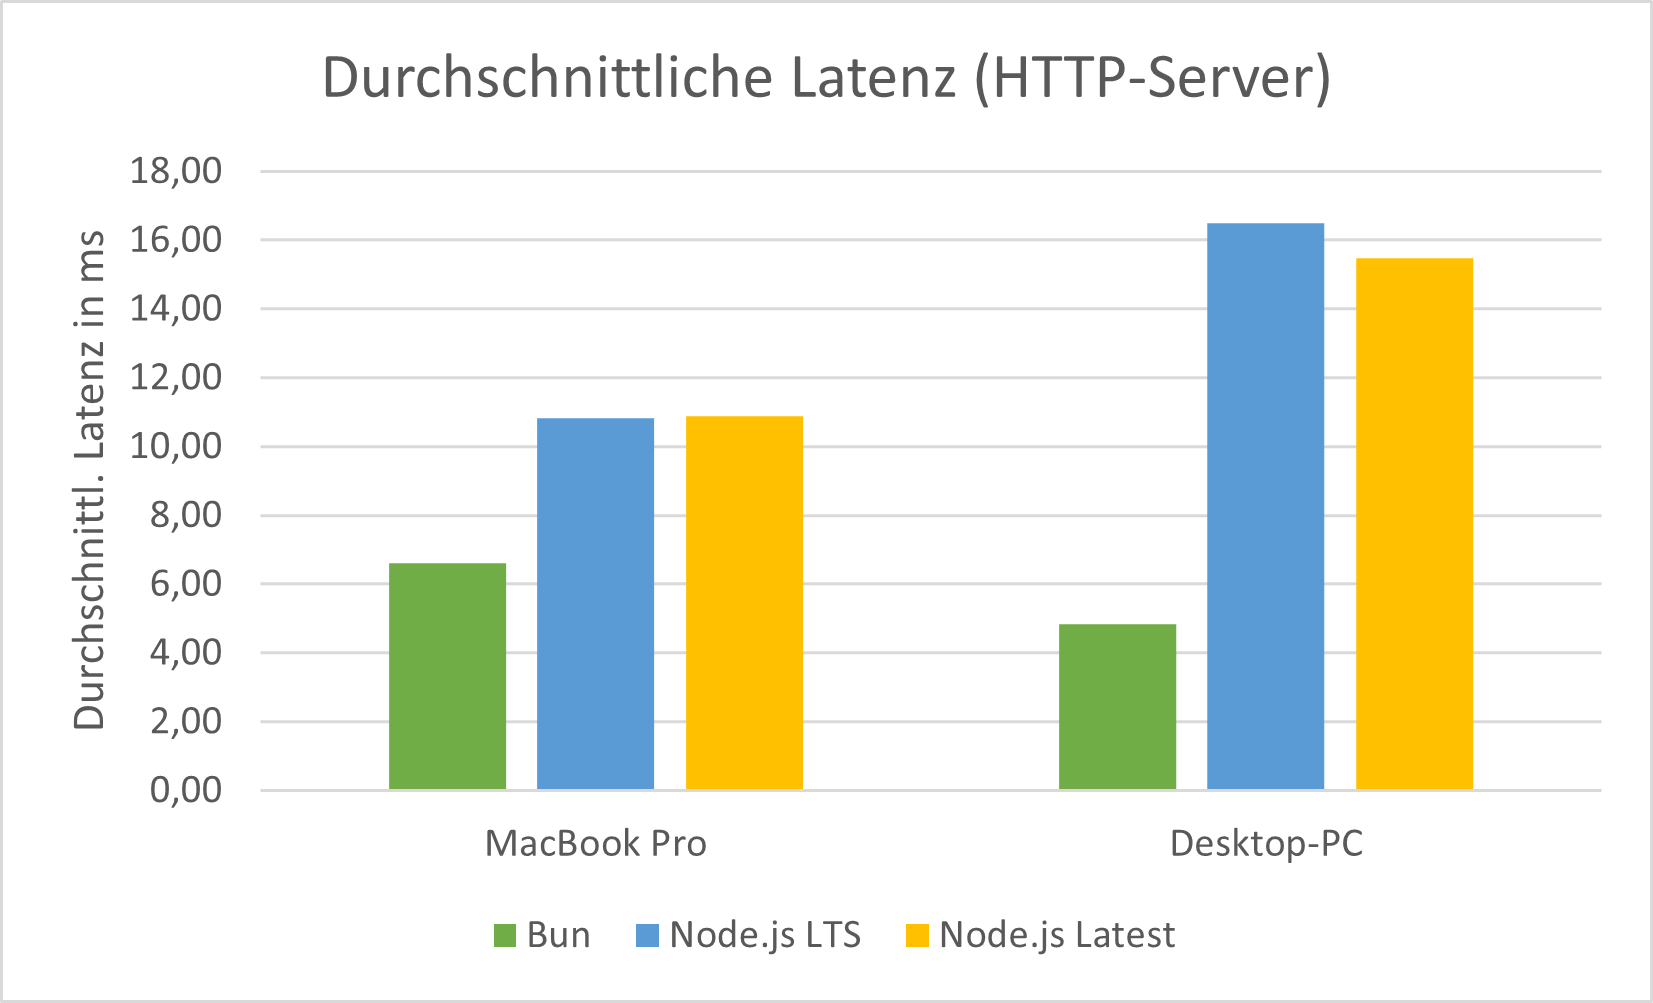
\includegraphics[width=\linewidth]{./images/httpServerAverageLatency.png}
	\caption{HTTP-Server - Durchschnittliche Latenz}
	\label{fig:httpServerAverageLatency}
	\textit{Quelle: Eigene Darstellung}
\end{figure}

